\pagestyle{quadrado}
\label{quadrado}

\begin{textblock*}{5.625in}(0pt,0pt)%
\vspace*{-1.45cm}
\hspace*{-1.8cm}\includegraphics*[width=112mm]{./imgs/QUADRADO.png}
\end{textblock*}

\pagebreak

\hspace{.5cm}

\begin{center}
\hspace*{-2.5cm}\raisebox{5.5cm}{\rotatebox[origin=t]{90}{\Formular{\textbf{Lançamento}}}}
\hspace*{2cm}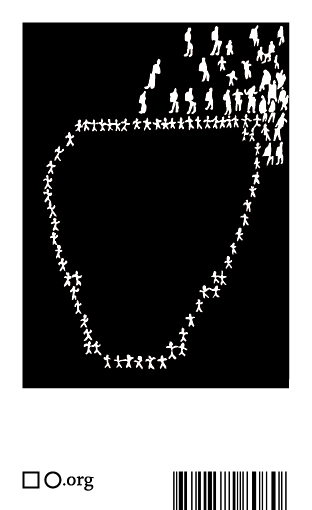
\includegraphics[width=45mm]{./imgs/fuga.png}
\end{center}

\hspace*{-2cm}\_\_\_\_\_\_\_\_\_\_\_\_\_\_\_\_\_\_\_\_\_\_\_\_\_\_\_\_\_\_\_\_\_\_\_\_\_\_\_\_\_\_\_\_\_\_\_\_\_\_\_\_\_\_\_\_\_\_\_\_\_\_\_\_\_\_\_\_\_\_\_\_\_\_

\medskip

\noindent{}Lorem ipsum dolor sit amet, consectetur adipiscing elit.
Donec sodales tortor a purus accumsan, ut ultricies purus
maximus. Aliquam bibendum consequat mi, sed commo-
do velit pellentesque id. Vivamus ultricies ligula in semper
sagittis. Donec mollis odio in lectus tristique, sed convallis
est interdum. Cras eget sem condimentum, pretium purus
eu, auctor.

\vfill

\hspace*{-.4cm}\begin{minipage}[c]{1\linewidth}
\small{
{\Formular{\textbf{
\hspace*{-.1cm}Título: Em rota de fuga: ensaios sobre medo, violência, escrita\\
Autor: Fábio Zuker\\ 
Editora: quadradocirculo\\
Páginas: 181\\
Formato: 11x18cm\\
Preço: R\$ 49,90\\
ISBN: 978-85-7715-621-4
}}}}
\end{minipage}


\pagebreak

\hspace{.5cm}

\begin{center}
\hspace*{-.5cm}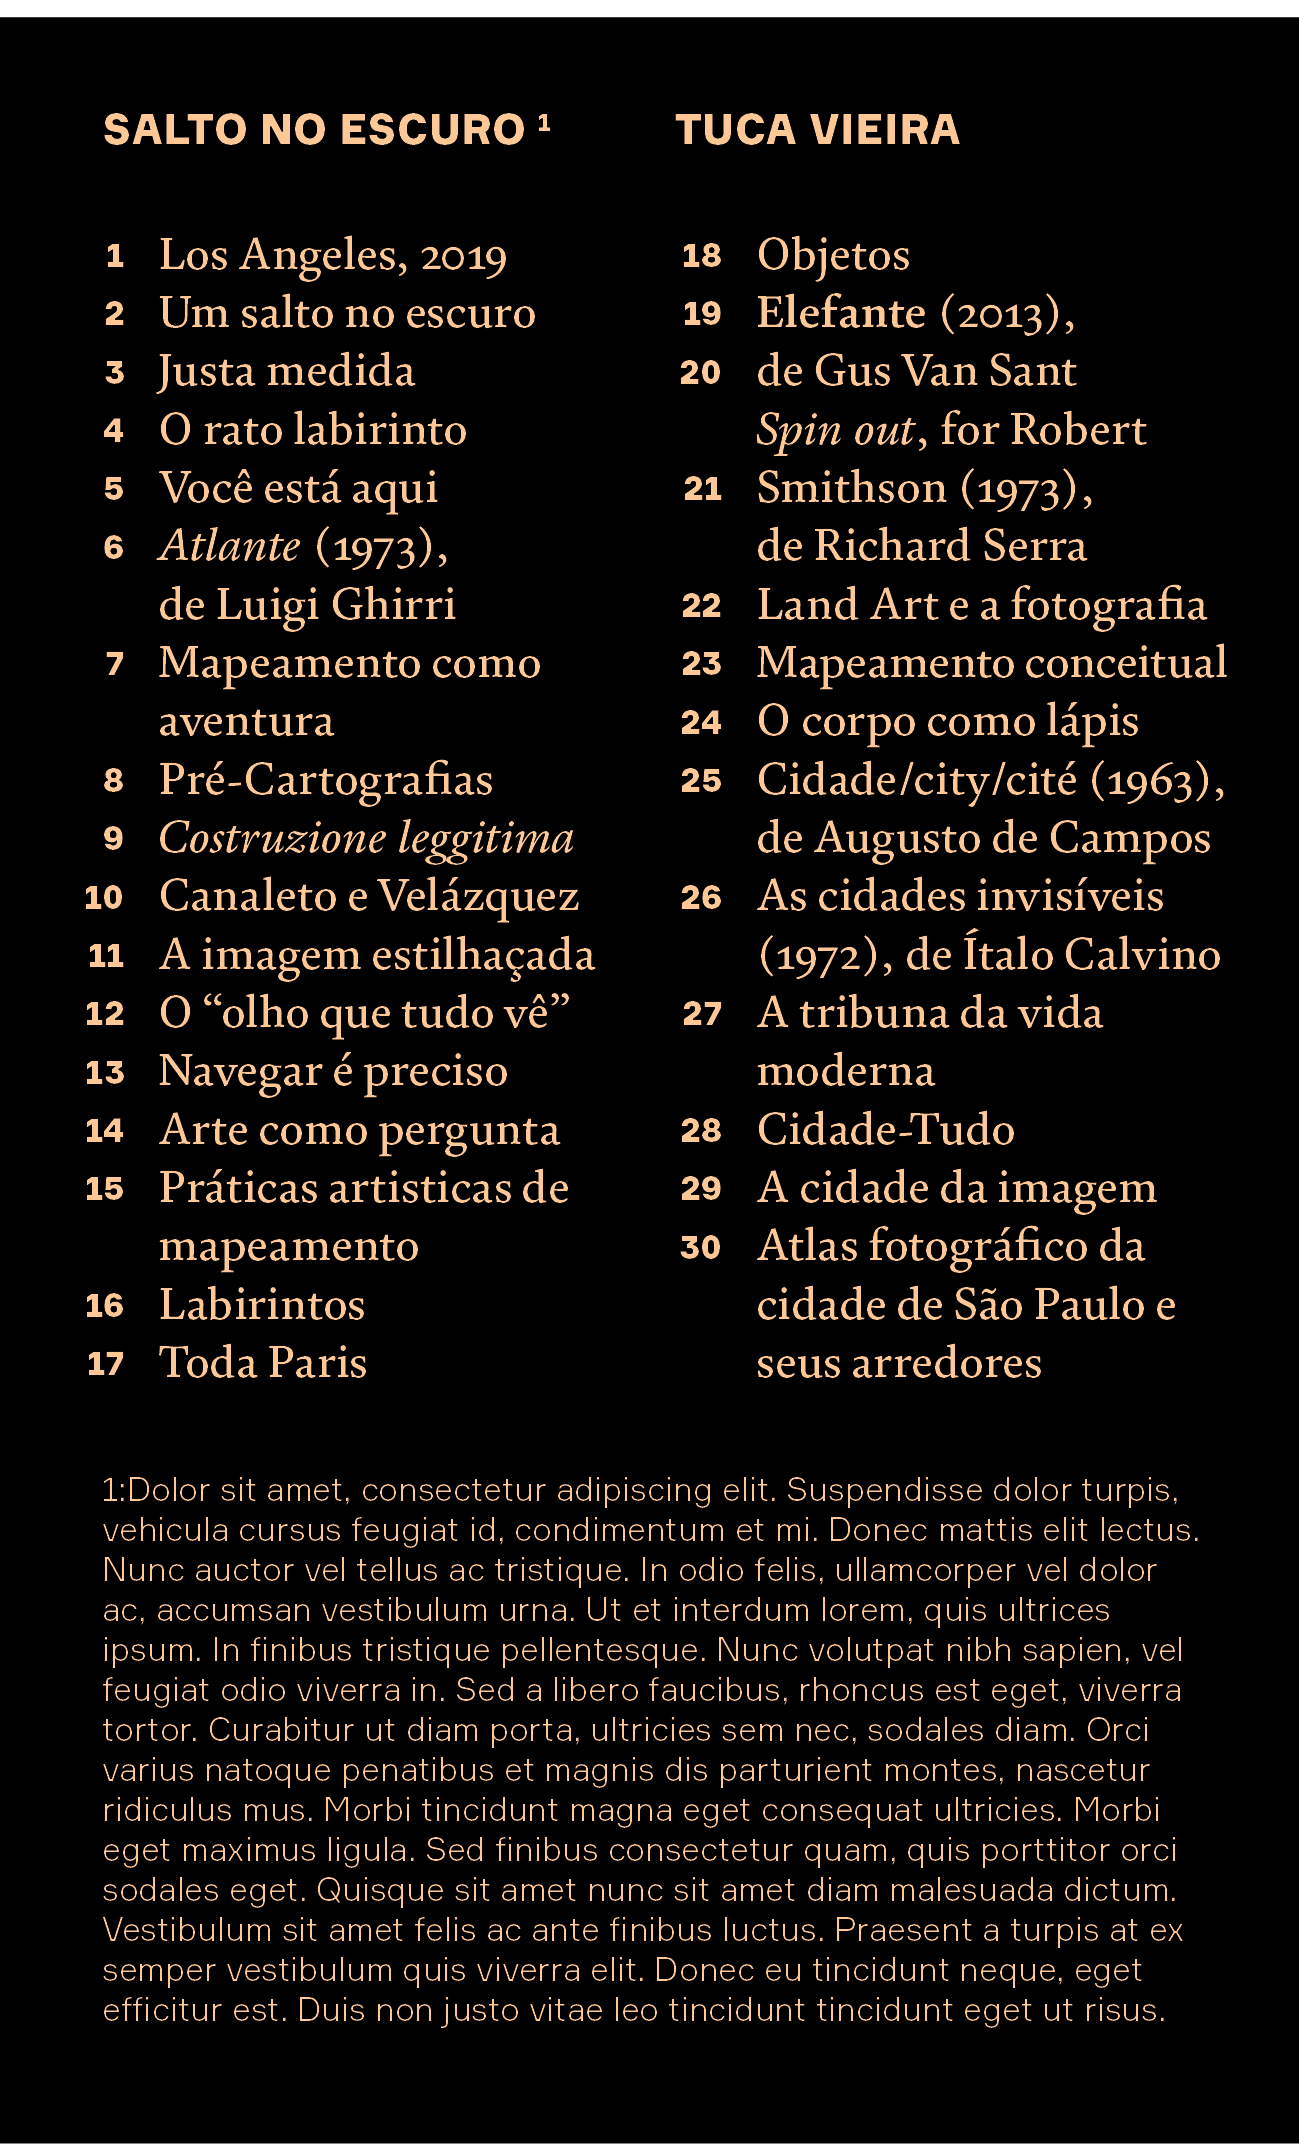
\includegraphics[width=45mm]{./imgs/escuro.png}
\end{center}

\hspace*{-2cm}\_\_\_\_\_\_\_\_\_\_\_\_\_\_\_\_\_\_\_\_\_\_\_\_\_\_\_\_\_\_\_\_\_\_\_\_\_\_\_\_\_\_\_\_\_\_\_\_\_\_\_\_\_\_\_\_\_\_\_\_\_\_\_\_\_\_\_\_\_\_\_\_\_\_

\medskip

\noindent{}Em {\slsc{Salto no escuro}}, o renomado fotógrafo Tuca Vieira percorre diversos centros urbanos, labirintos e criações artísticas para pensar o que é a cidade e o espaço geográfico contemporâneos. Marcado pela multiplicidade de caminhos, o autor instiga a novas possiblidades e percepções diante da aceleração da vida e da nova realidade impostas pela tecnologia. Como escreve, trata"-se de observar o abismo com o qual nos defrontamos, antes de saltar no escuro desses espaços mecânicos e artificiais.

\vfill

\hspace*{-.4cm}\begin{minipage}[c]{0.45\linewidth}
\small{
{\Formular{\textbf{
\hspace*{-.1cm}Título: Salto no escuro\\
Autor: Tuca Vieira\\ 
Editora: quadradocirculo\\
Páginas: 487\\
Formato: 11x18cm\\
Preço: R\$ 99,90\\
ISBN: 978-85-7715-622-1
}}}}
\end{minipage}

\pagebreak